% Fig. 4 -- Recording sessions and the three leakage-free evaluation
% protocols. Fill patterns (not colour) separate train / validation / test.
% Session sizes from splits/manifest.csv of the research repository.
\documentclass[tikz,border=2pt]{standalone}
\usepackage[T1]{fontenc}
\usepackage[scaled=0.92]{helvet}
\renewcommand{\familydefault}{\sfdefault}
\usetikzlibrary{patterns,positioning,calc}

\newcommand{\cellw}{13mm}
\newcommand{\cellh}{6mm}
% \cell{col}{row}{style}{text}
\newcommand{\cell}[4]{%
  \node[draw, line width=0.4pt, minimum width=\cellw, minimum height=\cellh,
        inner sep=0pt, #3] at ({(#1)*\cellw + ((#1)>4 ? 3mm : 0mm)}, {-(#2)*\cellh*1.25}) {#4};}

\begin{document}
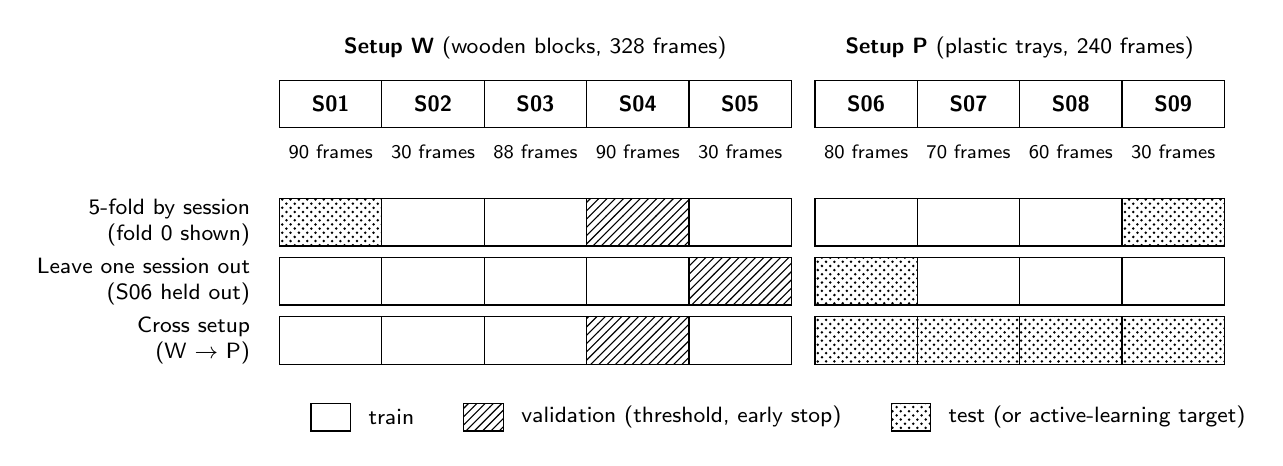
\begin{tikzpicture}[
  font=\footnotesize,
  tr/.style={fill=white},
  va/.style={pattern=north east lines},
  te/.style={pattern=crosshatch dots},
  no/.style={fill=black!12},
]
% ----------------------------------------------------------- header rows
\foreach \s/\n [count=\i from 0] in {S01/90,S02/30,S03/88,S04/90,S05/30,S06/80,S07/70,S08/60,S09/30}{
  \cell{\i}{0}{tr}{\textbf{\s}}
  \cell{\i}{0.8}{draw=none}{\scriptsize \n\ frames}
}
\node[anchor=south] at ({2*\cellw}, 0.45) {\textbf{Setup W} (wooden blocks, 328 frames)};
\node[anchor=south] at ({6.5*\cellw + 3mm}, 0.45) {\textbf{Setup P} (plastic trays, 240 frames)};

% ----------------------------------------------------------- k-fold (fold 0)
\node[anchor=east, align=right] at (-9mm, {-2*\cellh*1.25}) {5-fold by session\\(fold 0 shown)};
\foreach \i/\st in {0/te,1/tr,2/tr,3/va,4/tr,5/tr,6/tr,7/tr,8/te}{ \cell{\i}{2}{\st}{} }

% ----------------------------------------------------------- LOSO
\node[anchor=east, align=right] at (-9mm, {-3*\cellh*1.25}) {Leave one session out\\(S06 held out)};
\foreach \i/\st in {0/tr,1/tr,2/tr,3/tr,4/va,5/te,6/tr,7/tr,8/tr}{ \cell{\i}{3}{\st}{} }

% ----------------------------------------------------------- cross setup
\node[anchor=east, align=right] at (-9mm, {-4*\cellh*1.25}) {Cross setup\\(W $\rightarrow$ P)};
\foreach \i/\st in {0/tr,1/tr,2/tr,3/va,4/tr,5/te,6/te,7/te,8/te}{ \cell{\i}{4}{\st}{} }

% ----------------------------------------------------------- legend
\begin{scope}[shift={(0, {-5.3*\cellh*1.25})}]
  \node[draw, minimum width=5mm, minimum height=3.5mm, tr] (l1) at (0,0) {};
  \node[right=1mm of l1] (t1) {train};
  \node[draw, minimum width=5mm, minimum height=3.5mm, va, right=5mm of t1] (l2) {};
  \node[right=1mm of l2] (t2) {validation (threshold, early stop)};
  \node[draw, minimum width=5mm, minimum height=3.5mm, te, right=5mm of t2] (l3) {};
  \node[right=1mm of l3] {test (or active-learning target)};
\end{scope}
\end{tikzpicture}
\end{document}
